\documentclass[12pt]{article}
\usepackage[margin = 0.9in, top=0.8in]{geometry}
\usepackage{graphicx}
\usepackage{textgreek}
\usepackage{amsmath}
\usepackage{amsfonts}
\usepackage{mathtools}
\usepackage{amssymb}
\usepackage{float}
\usepackage{subcaption}
\usepackage{hyperref}
\usepackage{grffile}
\graphicspath{{./2/images},{./}}

\title{CS 754 - Advanced Image Processing\\Assignment 1 - Report}
\author{Shaan ul Haque - 180070053\\Mantri Krishna Sri Ipsit - 180070032}

\begin{document}

\maketitle

\section*{Question 1}
\subsection*{1.a}
We know that $\delta_{2s}$ is an increasing function of s(sparsity of signal). If we increase s, we are increasing $\delta_{2s}$ which in-turn increases $C_1$ and $C_2$ because they are increasing functions of $\delta_{2s}$ as well. Thus, both have conflicting effects so we can't assume the error bound to arbitrarily decrease as s increases. 
\subsection*{1.b}
Though, m(number of measurements) has no direct effect on the bound but it does have few implications on it. The measurement matrix has only m rows. If the sparsity of signal is s which is greater than m then we have:
\begin{equation*}
    \boldsymbol{y} = \sum_{i\epsilon\boldsymbol{S}}\boldsymbol{A_i}x_i
\end{equation*}
where $\boldsymbol{S}$ is the set of index where $\boldsymbol{x}$ has non-zero elements and $\boldsymbol{A_i}$ is the corresponding column. Now since s(cardinality of $\boldsymbol{S}$) is greater than m thus it is linear combination of s m-dimensional vectors which is clearly zero for some $\boldsymbol{x}$ as infinite solutions exists for such under-determined problem. Thus, the null set property of the matrix and hence RIP is lost. Thus, we must have m>s, as a necessary condition for RIP. Infact $O(slog(n/s))\leq m$, and thus the value of s cannot be increased beyond the number of rows in $\boldsymbol{A}$.
\subsection*{1.c}
Theorem 3 is better than theorem 3A. This is because a matrix obeying RIP for smaller bound on $\delta_{2s}$ would work fine on signals having more sparsity(smaller values of s) than a matrix whose RIC is larger. Thus, for larger $\delta_{2s}$ we can work with comparatively less sparse signals also and satisfy the BP error limit.
\subsection*{1.d}
If we make the error $\epsilon$ zero in BP, then we want exact relation between y and $\theta$ which is:
\begin{align*}
    y = \boldsymbol{\Phi\Psi\theta}
\end{align*}
But since the measurements are noisy in, the estimated $\theta$ from solving such problem would be incorrect. Thus, we allow some margin so that we do not over-fit our estimated $\theta$ with noisy measurements. Moreover, we see that $\epsilon$ is not some independent parameter but it depends upon the noise power, therefore it is quite unreasonable to take it as zero if noise vector is non-zero in magnitude.

\section*{Question 2}
\subsection*{2.a}
The first $T=3$ frames of the `cars' video are as follows:
\begin{figure}[ht]
	\centering
	\begin{minipage}[bt]{0.3\linewidth}
		\centering
		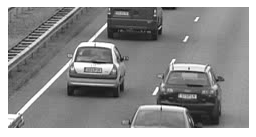
\includegraphics[scale=0.7]{cars_1.png}
		\caption{$T = 1$}
	\end{minipage}
\begin{minipage}[bt]{0.3\linewidth}
	\centering
	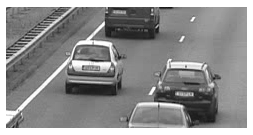
\includegraphics[scale=0.7]{cars_2.png}
	\caption{$T = 2$}
\end{minipage}
\begin{minipage}[bt]{0.3\linewidth}
	\centering
	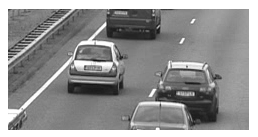
\includegraphics[scale=0.7]{cars_3.png}
	\caption{$T = 3$}
\end{minipage}
\end{figure}
\subsection*{2.b}
The coded snapshot for $T=3$ is as follows:
\begin{figure}[ht]
	\centering
	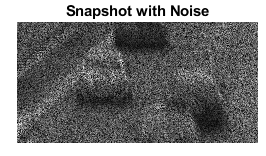
\includegraphics[scale=1]{3_coded_snapshot.png}
	\caption{Coded Snapshot along with Gaussian Noise with standard deviation 2}
\end{figure}
\subsection*{2.c}
We have
$$E_u = \sum \limits_{t=1}^TC_t \cdot F_t$$
Rewriting it as a matrix product and vectorizing the coded snapshot and the image to be measured, we get
$$\mathbf{b =  A\, x}$$
where
$$b = \text{Vectorized } E_u \in \mathbb{R}^{HW}$$
$$x = \text{Vectorized } F_u \in \mathbb{R}^{HWT}$$
$$A = [S_1|S_2|\cdots|S_T], S_t = \text{diag}(C_t(:)) \in \mathbb{R}^{HW \times HWT}$$
\subsection*{2.d}
Rewriting the above equation patchwise, we have
$$\mathbf{A\,x = b}$$
where
$$A = \Phi \Psi \in \mathbb{R}^{64\times 64T}$$
$$\Phi = [S_{i1}|S_{i2}|\cdots|S_{iT}], S_{it} = \text{diag}(C_{it}(:)) \in \mathbb{R}^{64 \times 64T}$$
$$\Psi = I_{T} \:\otimes \psi_{64,64} \: \otimes\: \psi_{64,64}$$
$$\psi_n = \text{2D DCT Basis Matrix of size } n \times n$$
$$x \in \mathbb{R}^{64T}, \text{ sparse}$$
$$b \in \mathbb{R}^{64}$$
Let $\theta^*$ be the optimal solution of the problem P0: $\min \: \left\lVert\theta\right\rVert_0$ such that $\left \lVert y - A \theta\right \rVert_2^2 \leq \epsilon, A = \Phi \Psi$.
Let the solution obtained using OMP be $\hat{\theta}$. Then we have the error as
\begin{eqnarray*}
E &=& \left \lVert \theta^* - \hat{\theta}\right \rVert^2\\
&=& (\theta^* - \hat{\theta})^T\: (\theta^* - \hat{\theta})\\
&=& (A^TA)^{-1} (A\theta^* - A\hat{\theta})^T \: (A\theta^* - A\hat{\theta})\\
&=& (A^TA)^{-1} \bigg((y - A\hat{\theta}) - (y - A\theta^*)\bigg)^T\: \bigg((y - A\hat{\theta}) - (y - A\theta^*)\bigg)\\
&=& (A^TA)^{-1}\: 4\epsilon\\
&=& \frac{4\epsilon}{\left\lVert A \right \rVert^2}
\end{eqnarray*}
\subsection*{2.e}
For $T=3$, the relative mean squared error that we obtained is 0.0112.
The reconstruction for $T=3$ is as follows:
\vspace{2cm}
\begin{center}
	\textit{Please turn over}
\end{center}
\newpage
\begin{figure}[ht]
	\centering
	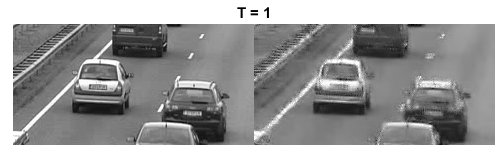
\includegraphics[scale=1]{3_1.png}
	\caption{$t = 1$, Left - Original, Right - Reconstructed}
\end{figure}
\begin{figure}[ht]
	\centering
	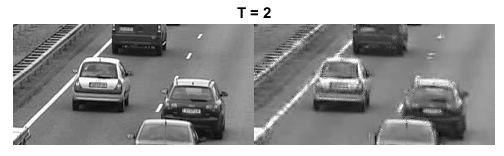
\includegraphics[scale=1]{3_2.png}
	\caption{$t = 2$, Left - Original, Right - Reconstructed}
\end{figure}
\begin{figure}[ht]
	\centering
	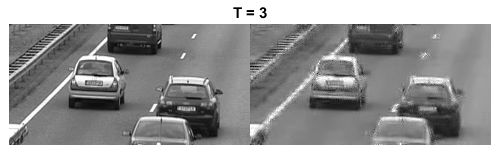
\includegraphics[scale=1]{3_3.png}
	\caption{$t = 3$, Left - Original, Right - Reconstructed}
\end{figure}
\subsection*{2.f}
The relative mean squared error value for $T = 5$ is 0.0194 and for $T = 7$ is 0.0316.
\vspace{2cm}
\begin{center}
\textit{Please turn over}
\end{center}
\newpage
\begin{figure}[ht]
	\centering
	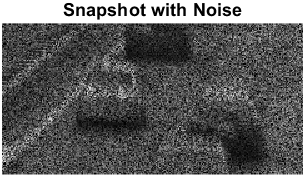
\includegraphics[scale=1]{5_coded_snapshot.png}
	\caption{Coded snapshot with noise for $T = 5$}
\end{figure}
\begin{figure}[ht]
	\centering
	\begin{minipage}[bt]{0.4\linewidth}
		\centering
			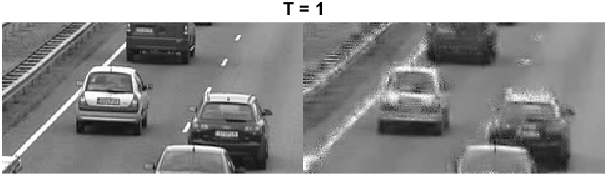
\includegraphics[scale=0.7]{5_1.png}
			\caption{$t = 1$}
			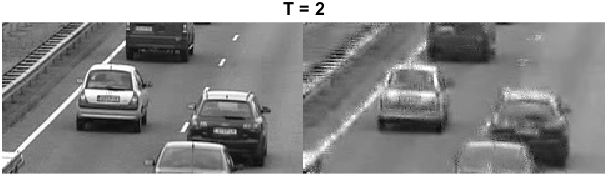
\includegraphics[scale=0.7]{5_2.png}
			\caption{$t = 2$}
			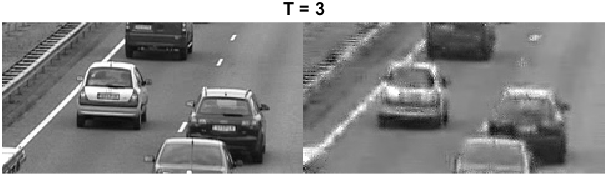
\includegraphics[scale=0.7]{5_3.png}
			\caption{$t = 3$}
	\end{minipage}
\begin{minipage}[bt]{0.5\linewidth}
\centering
	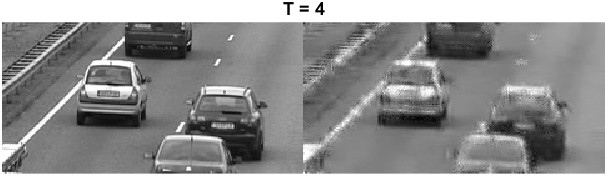
\includegraphics[scale=0.7]{5_4.png}
	\caption{$t = 4$}
	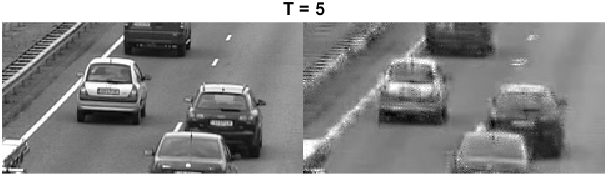
\includegraphics[scale=0.7]{5_5.png}
	\caption{$t = 5$}
\end{minipage}
\caption{Left - Original, Right - Reconstructed}
\end{figure}
\vspace{3cm}
\begin{center}
	\textit{Please turn over}
\end{center}
\newpage
\begin{figure}[ht]
	\centering
	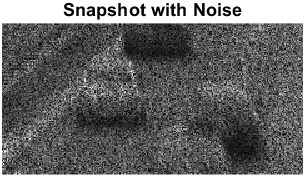
\includegraphics[scale=1]{7_coded_snapshot.png}
	\caption{Coded snapshot with noise for $T = 7$}
\end{figure}
\begin{figure}[ht]
\centering
\begin{minipage}[bt]{0.4\linewidth}
	\centering
	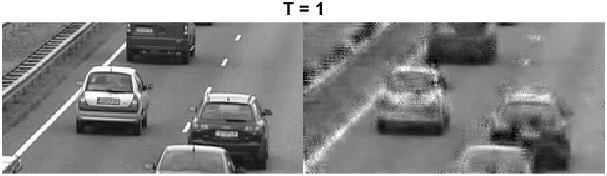
\includegraphics[scale=0.7]{7_1.png}
	\caption{$t = 1$}
	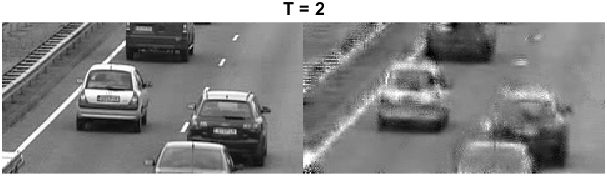
\includegraphics[scale=0.7]{7_2.png}
	\caption{$t = 2$}
	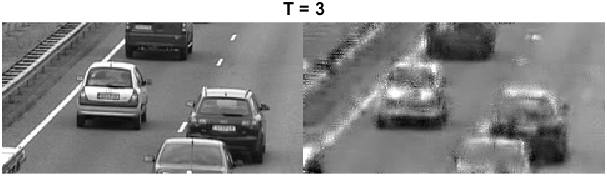
\includegraphics[scale=0.7]{7_3.png}
	\caption{$t = 3$}
	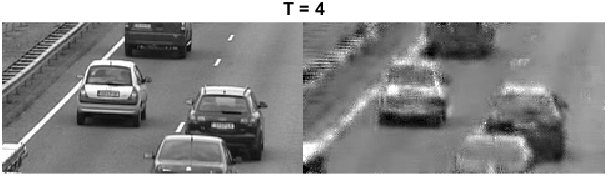
\includegraphics[scale=0.7]{7_4.png}
	\caption{$t = 4$}
\end{minipage}
\begin{minipage}[bt]{0.5\linewidth}
	\centering
	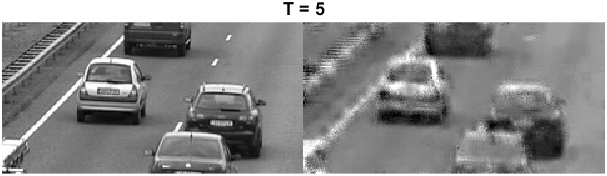
\includegraphics[scale=0.7]{7_5.png}
	\caption{$t = 5$}
	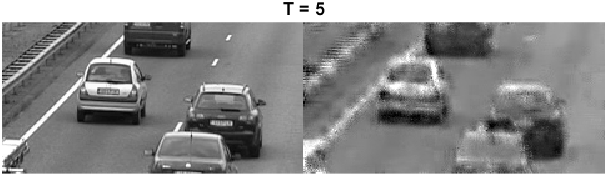
\includegraphics[scale=0.7]{7_6.png}
	\caption{$t = 6$}
	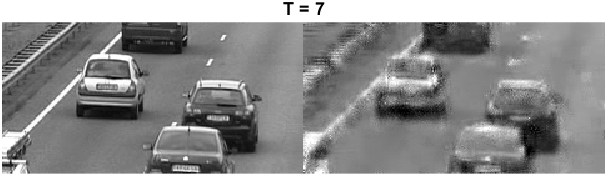
\includegraphics[scale=0.7]{7_7.png}
	\caption{$t = 7$}
\end{minipage}
\caption{Left - Original, Right - Reconstructed}
\end{figure}
\subsection*{2.g}
We have extracted a portion of about $120 \times 240$ around the lower right corner of every frame to save time. Hence, all our result correspond to this part. 
\newpage
\subsection*{2.h}
We have used the first 5 frames of the `flame' video to do the experiment. We got an relative mean squared error of 0.0010.
\begin{figure}[ht]
	\centering
	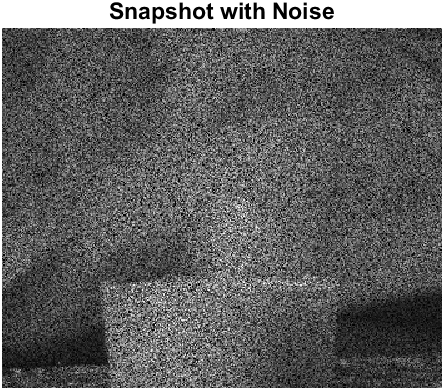
\includegraphics[scale=1]{flame_coded_snapshot.png}
	\caption{Coded snapshot for flame with noise for $T = 5$}
\end{figure}
\begin{figure}[ht]
	\centering
		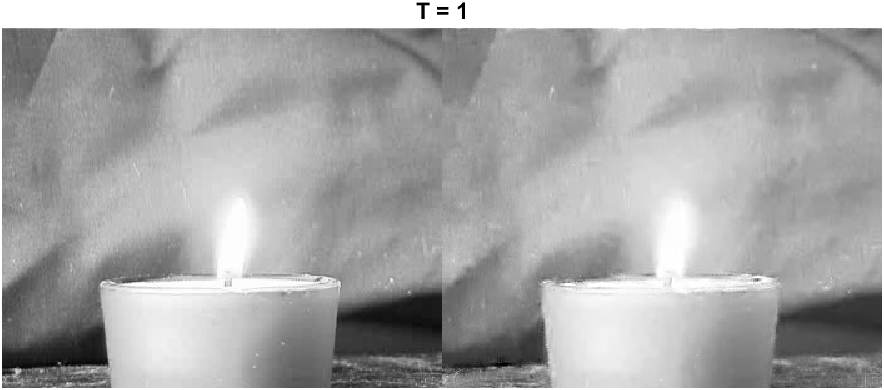
\includegraphics[scale=1]{flame_1.png}
		\caption{$t = 1$, Left - Original, Right - Reconstructed}
\end{figure}
\begin{figure}[ht]
	\centering
	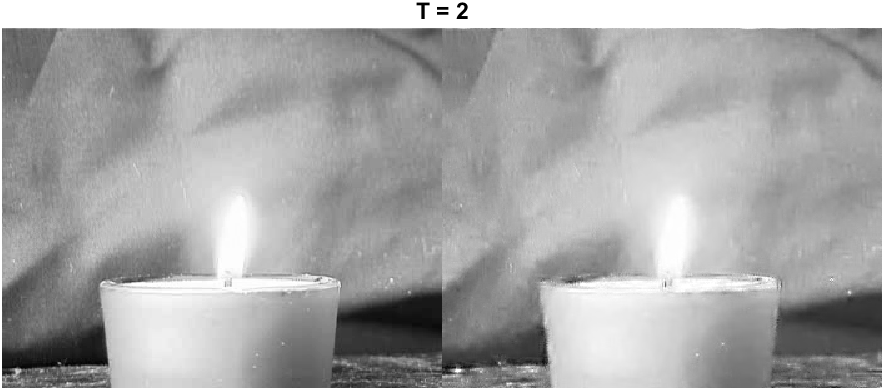
\includegraphics[scale=1]{flame_2.png}
	\caption{$t = 2$, Left - Original, Right - Reconstructed}
\end{figure}
\newpage
\begin{figure}[ht]
	\centering
	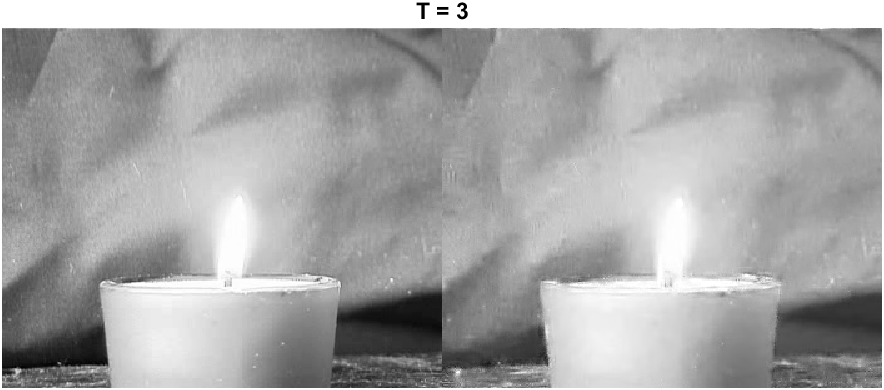
\includegraphics[scale=1]{flame_3.png}
	\caption{$t = 3$, Left - Original, Right - Reconstructed}
\end{figure}
\begin{figure}[ht]
	\centering
	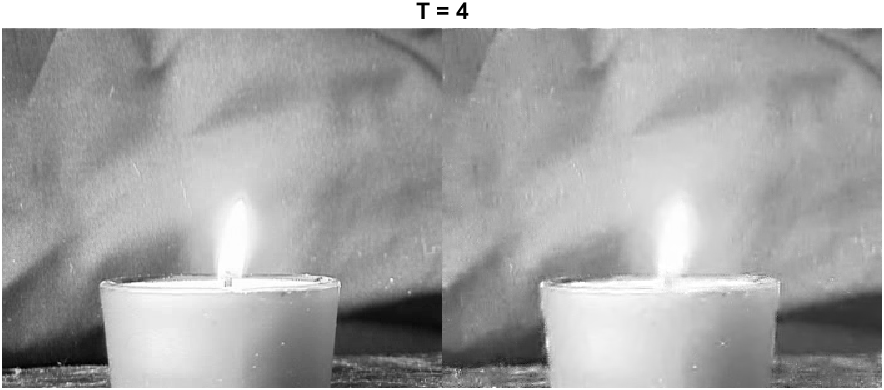
\includegraphics[scale=1]{flame_4.png}
	\caption{$t = 4$, Left - Original, Right - Reconstructed}
\end{figure}
\begin{figure}[ht]
	\centering
	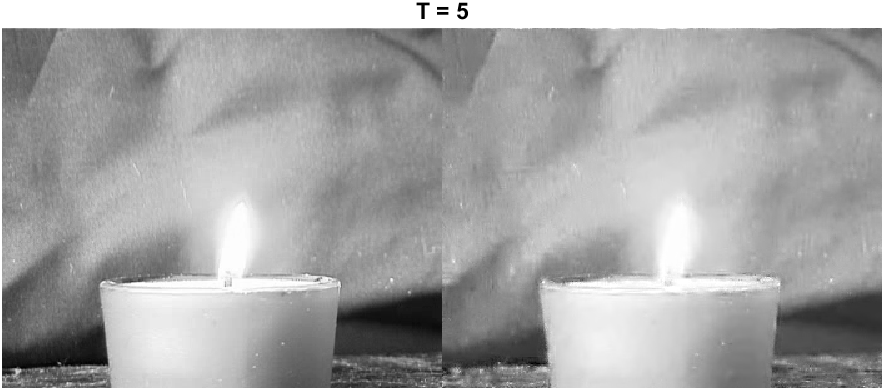
\includegraphics[scale=1]{flame_5.png}
	\caption{$t = 5$, Left - Original, Right - Reconstructed}
\end{figure}
\newpage
\section*{Question 3}
For upper limit of the bound, we can use Cauchy-Schwartz inequality:
\begin{equation*}
    |\boldsymbol{\Phi^i\Psi_j}| \leq |\boldsymbol{\Phi^i}||\boldsymbol{\Psi_j}|
\end{equation*}
which is simply dot product of two vectors is always less than product of their magnitude. Since $\boldsymbol{\Psi}$ and $\boldsymbol{\Phi}$ are unit normalized along columns and rows respectively we have:
\begin{equation*}
   \max_{i,j \epsilon \{1,2,3...,n\}}|\boldsymbol{\Phi^i\Psi_j}| \leq 1
\end{equation*}
And thus:
\begin{equation*}
   \max_{i,j \epsilon \{1,2,3...,n\}}\sqrt{n}|\boldsymbol{\Phi^i\Psi_j}| \leq \sqrt{n}
\end{equation*}
For lower limit of the bound, we use the hint by creating a unit vector:
\begin{equation*}
    \boldsymbol{g} = \sum_{k=1}^{n}\alpha_k\boldsymbol{\Psi_k}
\end{equation*}
Since $\boldsymbol{g}$ is a unit vector we have:
\begin{equation*}
    \boldsymbol{g^T}\boldsymbol{g} = (\sum_{k=1}^{n}\alpha_k\boldsymbol{\Psi_k^T})(\sum_{k=1}^{n}\alpha_k\boldsymbol{\Psi_k}) = 1
\end{equation*}
Now, since $\boldsymbol{\Psi}$ is orthonormal, dot product of columns of $\boldsymbol{\Psi}$ is zero when columns are different and equal to 1 if they are same. Thus we get the condition:
\begin{equation*}
     \sum_{k=1}^{n}\alpha_k^2 = 1
\end{equation*}
Now coherence between two matrices $\boldsymbol{\Phi}$ and $\boldsymbol{\Psi}$ is defined as the maximum value of dot product between row vectors of $\boldsymbol{\Phi}$ and column vectors of $\boldsymbol{\Psi}$. If we take $\boldsymbol{\Phi}$ to be a vector we need maximum dot product of the vector with the columns of $\boldsymbol{\Psi}$ which in other words is:
\begin{equation*}
    \mu(\boldsymbol{g}, \boldsymbol{\Psi}) = \max_{j \epsilon \{1,2,3...,n\}}\sqrt{n}\frac{|\boldsymbol{g^T\Psi_j}|}{\boldsymbol{||g||_2||\Psi_j||_2}}
\end{equation*}
Since $\boldsymbol{g}$ is a linear combination of columns of $\boldsymbol{\Psi}$ which is orthonormal also, we get:
\begin{equation*}
    \mu(\boldsymbol{g}, \boldsymbol{\Psi}) =  \max_{j \epsilon \{1,2,3...,n\}}\sqrt{n}\frac{|\alpha_j|}{||\boldsymbol{g||_2}}
\end{equation*}
The equation finally reduces to:
\begin{equation*}
    \mu(\boldsymbol{g}, \boldsymbol{\Psi}) =  \max_{j \epsilon \{1,2,3...,n\}}\sqrt{n}\frac{|\alpha_j|}{\sum_{k=1}^{n}\alpha_k^2} = \max_{j \epsilon \{1,2,3...,n\}}\sqrt{n}|\alpha_j|
\end{equation*}
The minimum value of the above expression can only be achieved when all the elements are equal which gives the lower limit of coherence:
\begin{equation*}
    n\alpha^2 = 1 \implies |\alpha| = 1/\sqrt{n}
\end{equation*}
This is very clear to see, let us assume if we decrease one of the parameters from $1/\sqrt{n}$ a little bit then other parameters will have to increase in order to satisfy the unit magnitude constraint and when max is taken across all elements then we will get some value greater than $1/\sqrt{n}$, whereas if we increase one of the parameters then others will have to decrease and max across all of them will again increase. Thus the minimum value is $\mu(\boldsymbol{g}, \boldsymbol{\Psi}) = 1$ when, $\boldsymbol{g} = 1/\sqrt{n}\sum_{k=1}^{n}\boldsymbol{\Psi_k}$

\section*{Question 4}
\subsection*{4.a}
If $\boldsymbol{x}$ is 1-sparse signal and only one measurement is taken then we won't be able to estimate $\boldsymbol{x}$ as we don't know which index element was non-zero. Whereas, if the index is known then the measurement can be divided by the value at the column of the measurement vector($n\times1$, as only one measurement is taken) corresponding to given index to uniquely determine $\boldsymbol{x}$.
\subsection*{4.b}
If two measurements are taken then also uniqueness is not guaranteed. Let us say some j-th index of $\boldsymbol{x}$ was non-zero while others were zero. Then we will get two measurements whose values are:
\begin{align*}
    m_1 = \Phi_{1j}x_j\\
    m_2 = \Phi_{2j}x_j
\end{align*}
If we divide the measurements we can get ratio of $\Phi_{1j}/\Phi_{2j}$ and check which column of $\boldsymbol{\Phi}$ has elements with this ratio. The problem is, that there might be more than one column satisfying this relation which will lead to many estimations of $x_j$ and hence compromising uniqueness.
\subsection*{4.c}
When $\boldsymbol{x}$ is 2-sparse and three measurements are taken, then let i-th and j-th element of signal have non-zero elements:
\begin{align*}
    m_1 = \Phi_{1i}x_i+\Phi_{1j}x_j\\
    m_2 = \Phi_{2i}x_i+\Phi_{2j}x_j\\
    m_3 = \Phi_{3i}x_i+\Phi_{3j}x_j
\end{align*}
This equation can be re-written in more readable form as:
\begin{align*}
    \begin{bmatrix} 
    m_1 \\
    m_2 \\
    m_3 \\
    \end{bmatrix} =
    \begin{bmatrix} 
    \Phi_{1i} \\
    \Phi_{2i} \\
    \Phi_{3i} \\
    \end{bmatrix}x_i +
    \begin{bmatrix} 
    \Phi_{1j} \\
    \Phi_{2j} \\
    \Phi_{3j} \\
    \end{bmatrix}x_j
\end{align*}
In other words, we need to check which two columns of $\boldsymbol{\Phi}$ are co-planar with the measurement vector. Since $\boldsymbol{\Phi}$ is randomly generated matrix the chance of more than two columns of $\boldsymbol{\Phi}$ to satisfy the condition exactly is less but in some cases there might be more than one solution for $\boldsymbol{x}$. Algorithm to determine $\boldsymbol{x}$ is:
\begin{verbatim}
1) Pick any two measurements say 1st and 2nd.
2) Loop over the columns of the matrix \Phi.
3) For any column p, pick any column q such that q>p, for all such q.
4) Solve the two linear equations for x_i and x_j with coefficients from the 
1st and 2nd row of \Phi_p and \Phi_q.
5) Put the calculated values in the third equation, i.e. with coefficients from 
the third row and check if the calculated value is equal to m_3.
\end{verbatim}
If more than two columns of $\boldsymbol{\Phi}$ pass the algorithm then $\boldsymbol{x}$ is not uniquely determinable. Otherwise, calculated $x_i$ and $x_j$ are the values with the column indices as their location in $\boldsymbol{x}$.
\subsection*{4.d}
When $\boldsymbol{x}$ is 2-sparse and four measurements are taken, then let i-th and j-th element of signal have non-zero elements:
\begin{align*}
    m_1 = \Phi_{1i}x_i+\Phi_{1j}x_j\\
    m_2 = \Phi_{2i}x_i+\Phi_{2j}x_j\\
    m_3 = \Phi_{3i}x_i+\Phi_{3j}x_j\\
    m_4 = \Phi_{4i}x_i+\Phi_{4j}x_j\\
\end{align*}
This equation can be re-written in more readable form as:
\begin{align*}
    \begin{bmatrix} 
    m_1 \\
    m_2 \\
    m_3 \\
    m_4 \\
    \end{bmatrix} =
    \begin{bmatrix} 
    \Phi_{1i} \\
    \Phi_{2i} \\
    \Phi_{3i} \\
    \Phi_{4i} \\
    \end{bmatrix}x_i +
    \begin{bmatrix} 
    \Phi_{1j} \\
    \Phi_{2j} \\
    \Phi_{3j} \\
    \Phi_{4j} \\
    \end{bmatrix}x_j
\end{align*}
In this case, the probability that more than two columns of $\boldsymbol{\Phi}$ satisfy the above condition is even more less. But in some bizarre cases we can encounter the situation that $\boldsymbol{x}$ is not unique. We have the same algorithm as used the previous part with only one more step, that is we should put the calculated values in the fourth linear equation also and check whether the calculated values satisfy it or not.
\section*{Question 5}
\subsection*{5.a}
Both the papers use sensors to compute coded snapshots. Hitomi's paper changes the code for each frame by sending signals to sensors directly whereas CACTI uses mechanical translation to compute a coded snapshot for several frames. Making uses of mechanics helps in reducing the power consumption and operating bandwidth of the camera. CACTI captures an object's spatiotemporal-multiplexed information. This mechanical translation helps in compressing temporal sampling without substantially increasing system volume or power. \\
The main difference between Hitomi's and CACTI is that Hitomi's paper tries to achieve  high spatial and spectral resolution whereas CACTI tries to achieve high spatial, spectral and temporal resolution by using the fact that the information present in natural images are highly correlated. In Hitomi's, the code/mask is fixed for an integration time whereas in CACTI, the mask changes continuously.
\newpage
\begin{figure}[ht]
	\centering
	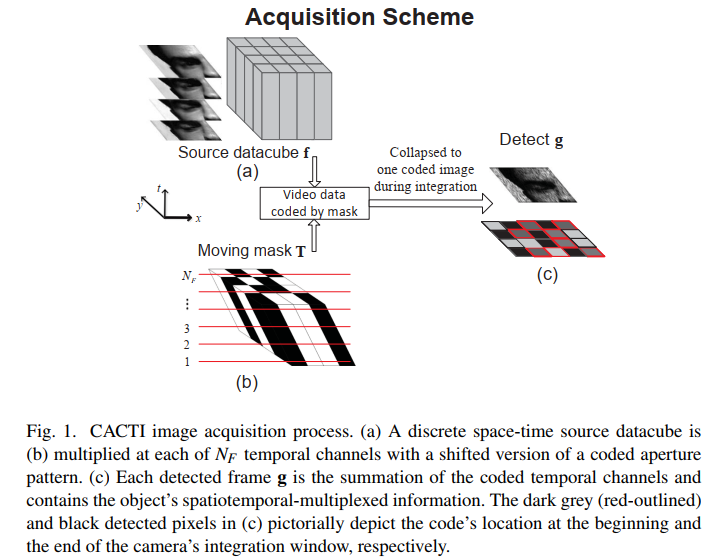
\includegraphics[scale=0.75]{CACTI.png}
	\caption{CACTI}
\end{figure}
\begin{figure}[ht]
	\centering
	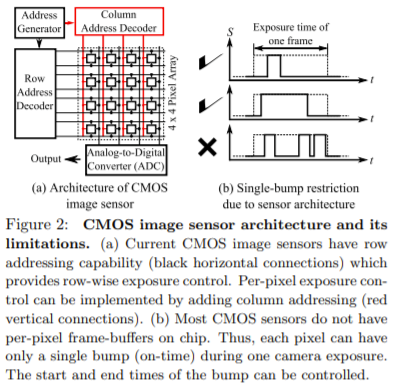
\includegraphics[scale=0.75]{Hitomi.png}
	\caption{Hitomi's}
\end{figure}
\subsection*{5.b}
This paper solves the following unconstrained optimization problem:
$$\arg \min_{\mathbf{f}}\left\lVert\mathbf{g - Hf}\right\rVert^2 + \lambda \mathbf{\Omega}(\mathbf{f}) $$
Here, for an $N$-pixel active sensor area, 
\begin{itemize}
\item $\mathbf{g} \in \mathbb{R}^N$ is the sensed data
\item $\mathbf{f} \in \mathbb{R}^{\sqrt{N} \times \sqrt{N} \times N_F}$ is a $(\sqrt{N} \times \sqrt{N}) \times N_F$ voxel spatiotemporal datacube i.e., the scene.
\item $\mathbf{H} \in \mathbb{R}^{N\times NN_F}$ s the system’s discrete forward matrix that accounts for sampling factors
including the optical impulse response, pixel sampling function, and time-varying transmission
function. The forward matrix is a 2-dimensional representation of the 3-dimensional transmission function $\mathbf{T}$
$$\mathbf{H}_k \stackrel{\text{def}}{=} \text{diag} \bigg[T_{1,1,k}, T_{2,1,k}, \cdots, T_{\sqrt{N}, \sqrt{N}, k}\bigg], \:\: k = 1, \ldots, N_F$$
$$\mathbf{H} \stackrel{\text{def}}{=} [\mathbf{H}_1\big| \mathbf{H}_2\big| \cdots \big| \mathbf{H}_{N_F} ]$$
\item $\lambda$ is a regularizer. This is chosen using experimental optimization.
\item $\mathbf{\Omega}(\mathbf{f})$ is the total variation of $\mathbf{f}$
$$\mathbf{\Omega}(\mathbf{f}) = \sum \limits_{k}^{N_F} \sum \limits_{i,j}^N \sqrt{(f_{i+1,j,k} - f_{i,j,k})^2 + (f_{i,j+1,k} - f_{i,j,k})^2}$$
\end{itemize} 
\section*{Question 6}
\subsection*{6.a}
\begin{itemize}
    \item Title - \textbf{Sparse imaging for fast electron microscopy}
    \item Authors - \textbf{Hyrum S. Anderson}, \textbf{ Jovana Ilic-Helms}, \textbf{Brandon Rohrer}, \textbf{Jason Wheeler} and \textbf{Kurt Larson}
    \item Place - \textbf{Sandia National Laboratories}
    \item Link - \href{https://cfwebprod.sandia.gov/cfdocs/CompResearch/docs/1210508c.pdf}{https://cfwebprod.sandia.gov/cfdocs/CompResearch/docs/1210508c.pdf}
\end{itemize}
\subsection*{6.b}
The scanning electron microscope acquires image by raster sampling (images in old phones or video games using dot matrix structure) focused electron beam. At each location, electrons in the incident beam interacts with sample, producing various signals about the composition or topography of the sample’s surface. These signals are  detected and digitally assigned to the image pixel value at the corresponding sample location. The electron probe is then repositioned via electromagnetic or electrostatic deflection to the subsequent pixel location.\\
In order to produce high-quality SEM images, long (on the order of microseconds) integration times per pixel are required to reduce noise. In many non-trivial cases detector response times and other factors necessitate very long integration time. In sum, well-engineered systems are SNR-limited in their data acquisition speed, and can require months to collect millimeters or centimeters of data for some applications.\\
The degrees of freedom of typical electron microscope images are many fewer than the number of image pixels. Hence, they focused the electron beam at random image points and acquired some M measurements, thereby reconstructing the image using BP.
\subsection*{6.c}
The reconstruction technique involves minimizing TVF norm with slight variation. The equations goes as:
\begin{align*}
    \boldsymbol{\textbf{y} = \Phi\textbf{x}+\textbf{n}}
\end{align*}
where \textbf{n} is noise vector $\bold\Phi$ is is a subset of rows of identity \textbf{I} and \textbf{n} is noise with power $\sigma^2$.
The image is obtained by solving regularized basis pursuit:
\begin{align*}
    \min_{x} \boldsymbol{||\Psi^Tx||_1 + ||\nabla x||_1}\\
    s.t. \ \boldsymbol{||y - \Phi x|| \leq  \sigma^2}
\end{align*}
 where  $\boldsymbol{||\nabla x||_1 = \sum_i\sqrt{|\nabla_hx_i|^2+|\nabla_vx_i|^2}}$. By the low mutual coherence
between the DCT basis and image-domain sampling, $\boldsymbol{\Psi}$ is chosen to be a block-DCT basis  with $32 \times 32$ pixel blocks. 
\end{document}
